\documentclass[]{article}
\usepackage{graphicx}
%opening

\title{Identifying macro-moths with micro-features}
\author{Paul J. Palmer}

\begin{document}

\maketitle

\begin{abstract}

This article explores the use of external microscopic features to support the identification (ID) of  macro-lepidoptera. The usual process of identifying macro-moths often focusses on the wings, which are often large and distinctively patterned. Matching an unknown specimen to reference pictures is often the identification method employed given the lack of systematic keys for Lepidoptera in general and coupled with experience, can give good results. The article uses a problematic identification as an example of how microscopic features may be used to narrow the field of candidate taxa to arrive at a specific taxon. 

\end{abstract}

\section*{A Difficult ID}
The specimen in question was taken at sugar 2020-08-16 on the Rutland Water Nature Reserve. It would have been recorded as a very worn example of Hypena proboscidalis (The Snout) if it had not briefly raised its wings in a posture uncharacteristic for this species, placing an element of doubt in this presumption. As can be seen in Figure~\ref{fig:202009131026pjp-1}, the specimen lacks long, forward pointing palps that give the Snout its vernacular name, buts its wings have the same slightly hooked shape (See Figure~\ref{fig:moth-at-sugar-hdr-2}), and similar median fascia. It would be easy to presume that the palps have been broken in what appears to be a worn specimen, but examination under magnification (Figure~) reveals that the palps are short and undamaged, which effectively eliminates Hypena proboscidalis as a candidate taxon for the speciment.

% TODO: \usepackage{graphicx} required
\begin{figure}
	\centering
	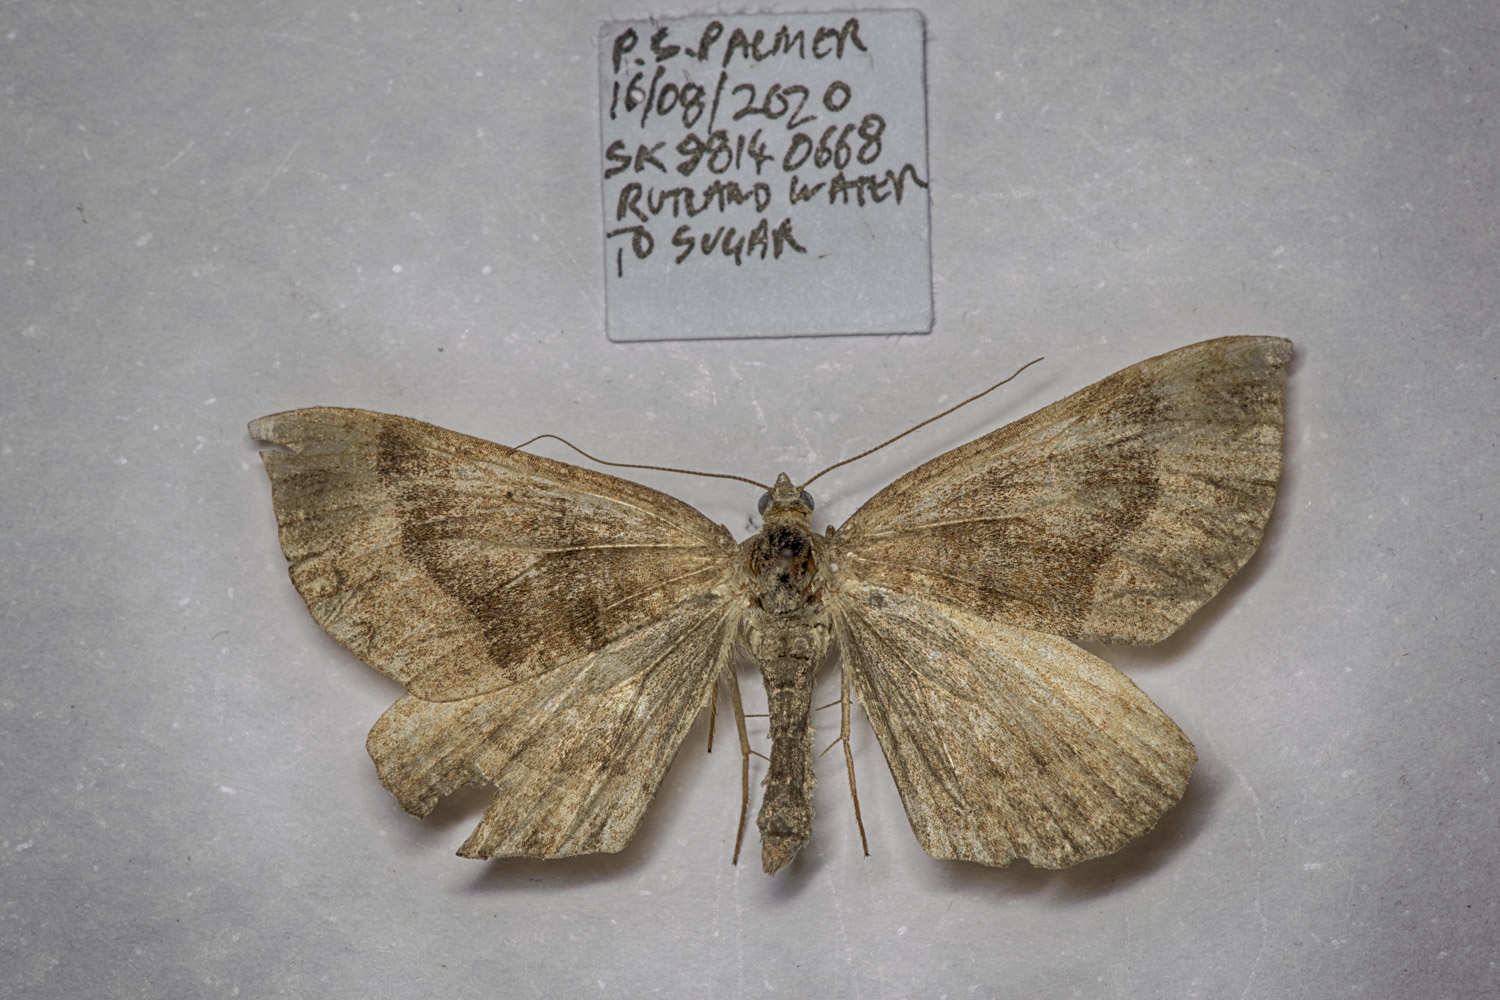
\includegraphics[width=0.5\linewidth]{images/202009131026PJP-1}
	\caption{Unkown specimen resembling Hypena proboscidalis.}
	\label{fig:202009131026pjp-1}
\end{figure}


\begin{figure}
	\centering
	\includegraphics[width=0.5\linewidth]{images/Moth-at-sugar-hdr-2}
	\caption{Hypena proboscidalis.}
	\label{fig:moth-at-sugar-hdr-2}
\end{figure}

\begin{figure}
	\centering
	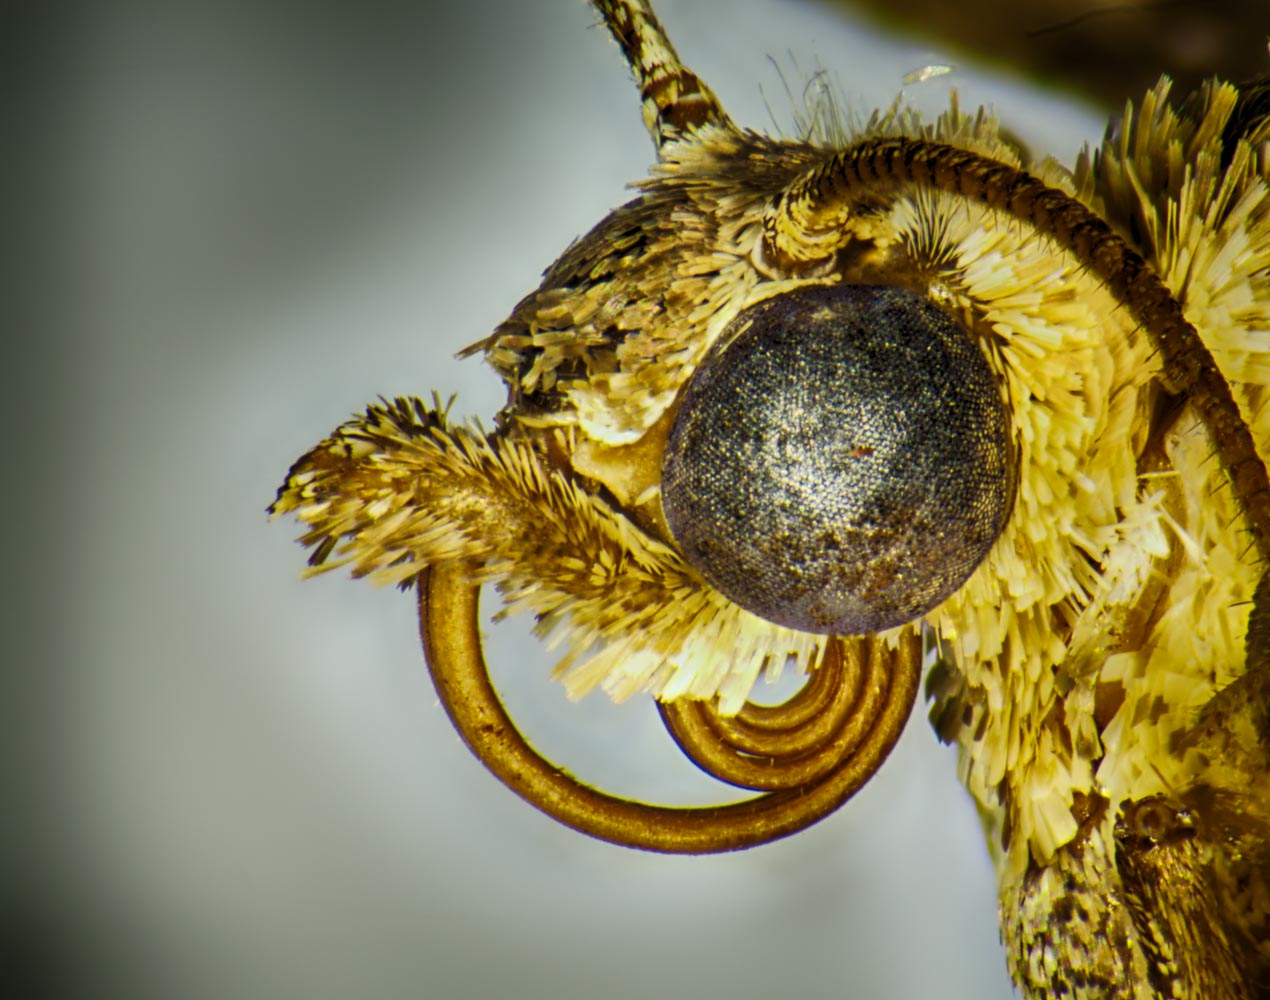
\includegraphics[width=0.5\linewidth]{images/20201112-1}
	\caption{Short undamaged palps eliminate Hypena proboscidalis as a candidate taxon.}
	\label{fig:20201112-1}
\end{figure}



\end{document}
